\documentclass[]{IEEEtran}

% Your packages go here
\usepackage[utf8]{inputenc}
\usepackage{graphicx}
\usepackage{float}
\usepackage{listings}
\usepackage{xcolor}
\usepackage{amsmath}
%listings settings
\definecolor{codegreen}{rgb}{0,0.6,0}
\definecolor{codegray}{rgb}{0.5,0.5,0.5}
\definecolor{codepurple}{rgb}{0.58,0,0.82}
\definecolor{backcolour}{rgb}{0.95,0.95,0.92}
\definecolor{codeblue}{rgb}{0,0.8,0.99}
\definecolor{codeyellow}{rgb}{0.6,0.5,0}


\lstdefinestyle{vim_like}{
  backgroundcolor=\color{backcolour},   
  commentstyle=\color{codegreen},
  keywordstyle=\color{codeyellow},
  numberstyle=\tiny\color{codegray},
  stringstyle=\color{codepurple},
  basicstyle=\ttfamily\footnotesize,
  breakatwhitespace=false,         
  breaklines=true,                 
  captionpos=b,                    
  keepspaces=true,                 
  numbers=left,                    
  numbersep=5pt,                  
  showspaces=false,                
  showstringspaces=false,
  showtabs=false,                  
  tabsize=2
}
\lstset{style=vim_like}

\newcommand\todolist[1]{\textcolor{red}{#1}}

\markboth{MC949/MO446 Computer Vision}{}

\begin{document}
  \title{Project 2 - Augmented Reality}
  \author{Iury Cleveston (RA 230216), Leonardo Rezende (RA 262953) and Thales Oliveira (RA 148051)
    \thanks{ra230216@students.ic.unicamp.br, ra262953@students.ic.unicamp.br, ra148051@students.ic.unicamp.br}
  }
  \maketitle
  
  \begin{abstract}
    In this project, we were given the task of performing Augmented Reality (AR) task in media, in this case, a video. The goal was to make an image appear in every single frame of the video, in this case, a specific target on the video is always substituted by the image, while the camera changes position, orientation and focal distance. In order to fulfill the requirements, the algorithm implemented deals with image descriptors for every frame pair to find the target, a matching algorithm to hypothesize matches and a RANSAC with least squares methodology to calculate the transform between frames. We were able to generate AR video, and the limitations of our implementation are explained in this report.
  \end{abstract}
  
\section{Introduction}
This work, developed by Group 8 of Computer Vision Course (2nd Semester/2019), has the goal of generating Augmented Reality videos, using a simple approach. In this sense, it is desired to substitute, in every single frame of the video, a specific region, which is called in this work "target", by another image, considering that the camera is moving freely in the environment (changing horizontal/vertical positions, rotating (counter)clockwise, zooming-in/out). To do such tasks, a pipeline was implemented and every single task divided. An image descriptor algorithm was implemented, to be able to locate the target frame within a video frame. For matching the target frame between 2 consecutive frames, a matching algorithm was implemented, to map candidate keypoints between those frames. Using those candidate matches, an algorithm using RANSAC and Least Squares was implemented to find the affine transform between frames. Therefore, we generate an AR video based on the original video, the descriptor, the matching algorithm and the affine transform algorithm. The following sections explain the implemented work, and the tests applied to the code.  

\section{Implemented Algorithm}
In this section, it is presented the implemented algorithm in this project. The code is distributed into five principal Python files, named \textbf{affine\_transform.py}, \textbf{ar.py}, \textbf{main.py}, \textbf{matching.py} and \textbf{sift.py}. The \textbf{affine\_transform.py} file contains the \textit{AffineTransform} class, which implements the RANSAC with Least Squares to calculate best Affine transform for the candidate matches. The \textbf{ar.py} file contains the \textit{AR} class, which implements the video manipulation, calls for the descriptor, matching and affine transform functions and pasting image into the target. The \textbf{main.py} file does the calls to the \textit{AR} class. The \textbf{matching.py} contains the \textit{Matching} class, which calculates possible candidate matches from the keypoints and its descriptions calculated by the implementation done in the \textbf{sift.py} file. The following subsections explains main implementation decisions done in key parts of the project, based on pipeline execution order.


\subsection{Implementation of the Pipeline}
\todolist{Explicar o arquivo AR}


\subsection{Find interest points in a pair of frames}
\todolist{Explicar o SIFT nosso}


\subsection{Matching keypoints between two frames}

To find the descriptors between two frames, we use the k-nearest neighbors (KNN) algorithm, this algorithm is widely used in the machine learning community and serves to detect similarities between objects. In this work, KNN was used to detect similarity between descriptors in different frames.

The algorithm takes as parameter two descriptor vectors from SIFT and returns an index vector, also known as matches, which will be used to later retrieve keypoints in the two frames. In our implementation, KNN was used to find 2 clusters, as shown in Listing~\ref{code:least-squares}.


 \begin{lstlisting}[language=Python, caption={K-nearest neighbors}, label={code:knn}]
 def _knn_match(self, query, train, k):
    """
    Perform the match using knn

    Keyword arguments:
    query -- the query vector
    train -- the training vector
    k -- number of clusters
    """

    matches = []

    # For each descriptor in the current
    for i, q in enumerate(query):

        # Get the k-nearest neighbors
        neighbor = self._get_neighbors(train, q, k)

        matches_knn = set()

        # Create the k descriptor tuple
        for n in neighbor:
            matches_knn.add(Match(i, n[0], n[1]))

        matches.append(matches_knn)

    return matches

def _get_neighbors(self, query, train, k):
    """
    Get the k-nearest neighbors

    Keyword arguments:
    query -- the query vector
    train -- the training vector
    k -- number of clusters
    """

    # Create the matrix of distances
    distances = np.zeros((np.shape(query)[0], 2), dtype=np.int)

    # For each pair, calculates the distance
    for x, q in enumerate(query):
        distances[x] = (x, euclidean_distance(train, q))

    # Sort based on distance using numpy notation
    distances = distances[distances[:, 1].argsort()]

    neighbors = []

    # Group in k clusteres
    for x in range(k):
        neighbors.append(distances[x])

    return neighbors
    
\end{lstlisting}

However, to compare points, one should use a distance metric. As we use SIFT to describe the points, the metric used was the distance $L_2$. In this implementation, we performed Hamming distance tests for BRIEF descriptors but chose to follow using SIFT.

The option for 2 clusters was made from the SIFT documentation, where the author, Lowe, uses a threshold of 0.75 between the two clusters to verify the quality of the matches, as shown in Listing~\ref{code:matching}.

\begin{lstlisting}[language=Python, caption={Matching Lowe's Criteria}, label={code:matching}]

def match(self, query, train, k=2):
    """
    Match the query with the train using k-nearest neighbors

    Keyword arguments:
    query -- the query vector
    train -- the training vector
    k -- number of clusters
    """

    matches_knn = self._knn_match(query, train, k)

    # Apply ratio test
    matches = []
    for m, n in matches_knn:
        if m.distance < 0.75*n.distance:
            matches.append(m)

    return matches

\end{lstlisting}

In addition, a class called \textbf{Match()} was implemented to store the similarity between descriptors, as shown in Listing~\ref{code:match}. This class is composed of the indexes of both descriptors and a distance value for them.

\begin{lstlisting}[language=Python, caption={Match Class}, label={code:match}]

class Match:
    """
       A class used to store the match information

       Methods
       -------
       """

    def __init__(self, queryIdx, trainIdx, distance):
        self.queryIdx = queryIdx
        self.trainIdx = trainIdx
        self.distance = distance

\end{lstlisting}

After implementing this code we ran several tests to validate the quality of the results. Below are shown two examples of matches between frames. Figure~\ref{fig:matches_0} shows the matches between the artificial frame and the first frame of the video.

\begin{figure}[H]
     \centering
     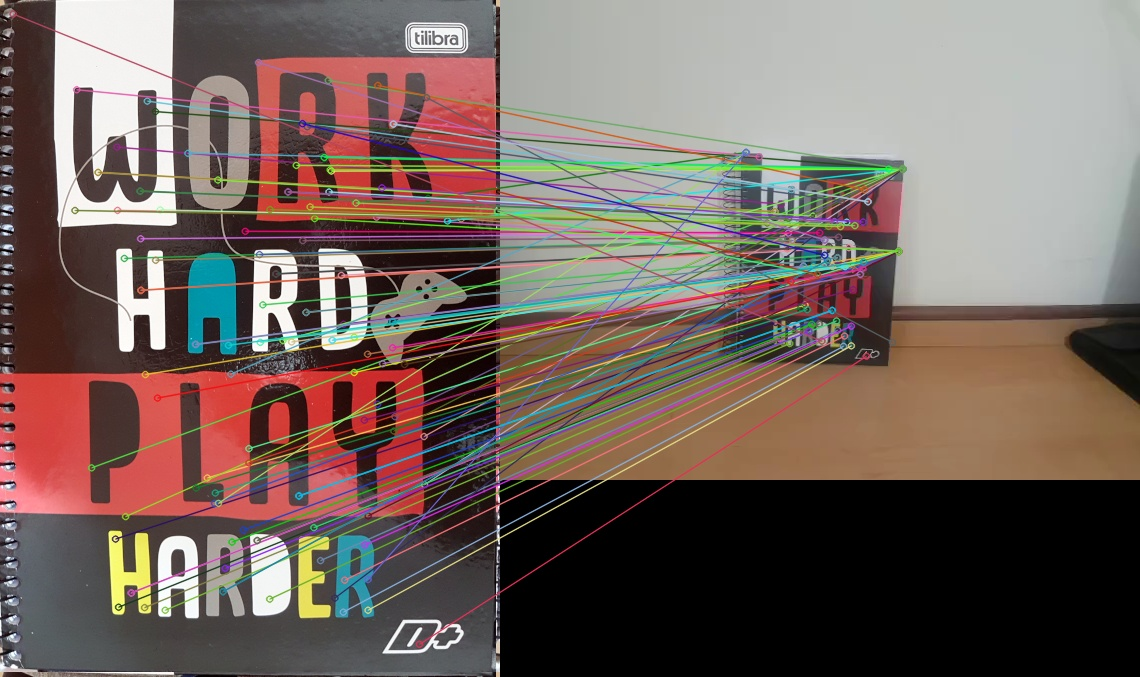
\includegraphics[width=0.9\hsize]{img/matches_0.jpg}
     \caption{Matches between the artifical frame and frame 0.}
     \label{fig:matches_0}
\end{figure}

In Figure~\ref{fig:matches_1} we can see the matches between two frames of the video.

\begin{figure}[H]
     \centering
     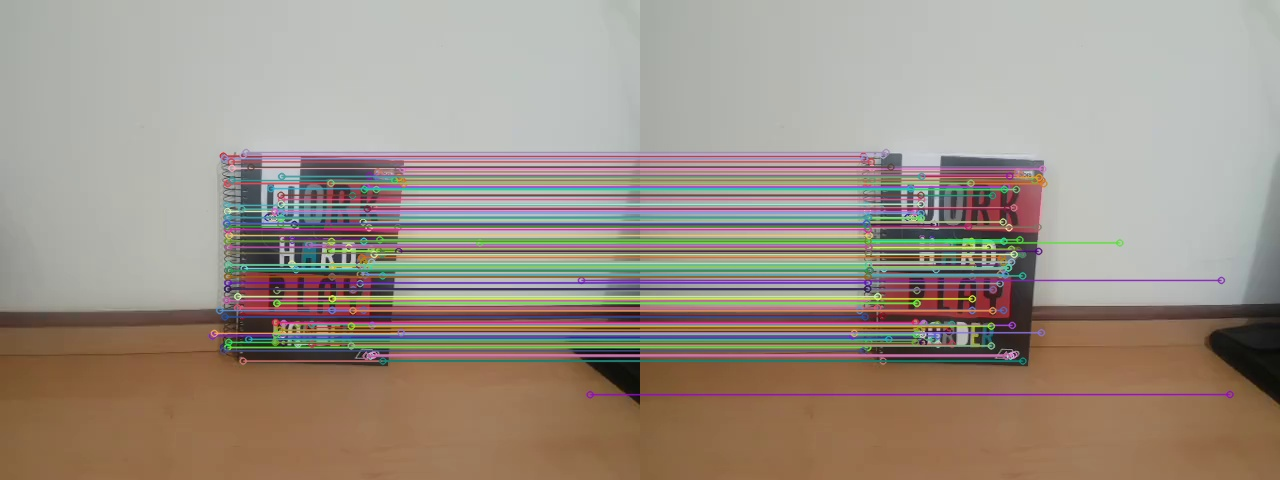
\includegraphics[width=0.9\hsize]{img/matches_1.jpg}
      \caption{Matches between frame 0 and frame 1.}
     \label{fig:matches_1}
\end{figure}

Therefore, the SIFT algorithm was able to detected the same points in both frames and the matching algorithm was able to select them based on their $L_2$ distance. The points are located in regions where the gradient is high, such as the notebook's borders, the letters and regions of high variation. Some points were also located in the wall and in the table, but they were the outliers.


\subsection{Calculating the Affine Transform between two frames}

To learn the appropriate Affine transform between frames, which is used for estimate the position of the target frame, the candidate keypoint matches from the previous subsection are used here. As the Affine transform has 6 degrees of freedom (associated with rotation and translation in the coordinate system), we need 3 pairs of candidate keypoints in order to find the parameters of the Affine transform matrix such that:

\begin{equation}
    Y = AX
    \label{eq:mat}
\end{equation}

which $Y$ are the candidate match points in the current frame, $A$ is the affine transform matrix and $X$ are the candidate match points in the previous frame. 
Equation \ref{eq:mat} can be explanded for the transformation of one pair of candidate matches as:

\begin{equation}
\begin{bmatrix}
  x_{i}^{'} \\ y_{i}^{'}
\end{bmatrix}  =
\begin{bmatrix}
  a & b & c \\ d & e & f
\end{bmatrix}.
\begin{bmatrix}
  x_{i} \\ y_{i} \\ 1
\end{bmatrix}  
\end{equation}

As we have 6 variables to solve for, we need 3 pairs of candidate matches.

To solve $A$ for three candidate matches, consider equation \ref{eq:mat}. Expanding the equation, we have that:

\begin{equation}
  \begin{bmatrix}
    x_{1} & y_{1} & 1 & 0 & 0 & 0 \\
    0 & 0 & 0 & x_{1} & y_{1} & 1 \\
    x_{2} & y_{2} & 1 & 0 & 0 & 0 \\
    0 & 0 & 0 & x_{2} & y_{2} & 1 \\
    x_{3} & y_{3} & 1 & 0 & 0 & 0 \\
    0 & 0 & 0 & x_{3} & y_{3} & 1 \\
  \end{bmatrix}
  .
  \begin{bmatrix}
      a \\
      b \\
      c \\
      d \\
      e \\
      f
  \end{bmatrix} = 
  \begin{bmatrix}
    x_{1}^{'} \\
    y_{1}^{'} \\
    x_{2}^{'} \\
    y_{2}^{'} \\
    x_{3}^{'} \\
    y_{3}^{'} \\
  \end{bmatrix}
\end{equation}

Using Least Squares for this specific case, we have that A is:

\begin{equation}
  A = (X^{T}X)^{-1}(X^{T}Y)
  \label{eq:ls}
\end{equation}

Listing \ref{code:least-squares} shows our implementation of the Least Squares to solve equation \ref{eq:ls}. As visible, we treat the possibility of $X^{T}.X$ being a singular matrix by returning A as a 0-matrix (bad combination of candidate matches).

 \begin{lstlisting}[language=Python, caption={Least Squares Implementation}, label={code:least-squares}]
  def least_squares(prev_points, curr_points):
    """
    It calculates least squares in order to find affine transform that transforms
    a set of coordinates to another

    Keyword arguments:
    prev_points -- set of original coordinates
    curr_points -- set of transformed coordinates
    """
    n_points = prev_points.shape[0]
    x = np.zeros(shape=(2*n_points, 6), dtype=np.float32)
    for idx, _ in enumerate(prev_points):
        x[2*idx] = [prev_points[idx][0], prev_points[idx][1], 1, 0, 0, 0]
        x[2*idx + 1] = [0, 0, 0, prev_points[idx][0], prev_points[idx][1], 1]

    y = np.zeros(shape=(2*n_points, 1), dtype=np.float32)
    for idx, _ in enumerate(curr_points):
        y[2*idx][0] = curr_points[idx][0]
        y[2*idx + 1][0] = curr_points[idx][1]

    transp_times_x = (np.transpose(x)).dot(x)
    det = np.linalg.det(transp_times_x)

    #Singular Matrix
    if det == 0:
        return np.zeros((6, 1))

    a = (np.linalg.inv(transp_times_x)).dot(((np.transpose(x)).dot(y)))
    return a
\end{lstlisting}

Considering that not necessarily all the candidates are suitable (as mentioned before), we use RANSAC (Random Sample Consensus) to estimate valid candidates for solving the system. This algorithm picks 3 random candidate matches, solves the $A$ matrix using Least Squares and evaluates if $A$ is good by testing it with the candidates themselves. If the calculated $A$ is the best, it holds that $A$. It executes the algorithm $k$ times, removing bad matches from the candidates to be picked to solve $A$ after every good $A$ fit. After $k$ times, it executes Least Squares algorithm one last time to all remaining match candidates to find best possible $A$ for the set, and returns it. Following subsections explain in a more detailed way the full implementation. The RANSAC algorithm explained here is shown in listing \ref{code:ransac}

\begin{lstlisting}[language=Python, caption={RANSAC to estimate Affine Transformation Matrix}, label={code:ransac}]
  def get_affine_transform_matrix(self, previous_f_points, current_f_points):
    """
    It runs RANSAC with least squares to find the affine transform
    matrix for the candidate matches

    Keyword arguments:
    previous_points -- set of original candidate coordinates
    current_points -- set of transformed candidate coordinates
    """
    point_matches = np.zeros((self._n_ransac_iterations, 3, 2), dtype=np.float32)
    best_number_matches = 0
    best_a = []
    previous_f_ransac_set = np.copy(previous_f_points)
    current_f_ransac_set = np.copy(current_f_points)

    # starts RANSAC
    for i in range(self._n_ransac_iterations):
        n_points = len(previous_f_ransac_set)
        # find 3-points combination which was not chosen before
        valid_eq_points = False
        while not valid_eq_points:

            idx = 0
            pf_guess_array = np.full((3, 2), -1)
            cf_guess_array = np.full((3, 2), -1)
            while idx < 3:

                guess = random.randint(0, n_points - 1)
                #if not guess in guess_array:
                if not (pf_guess_array == previous_f_ransac_set[guess]).all(1).any():
                    pf_guess_array[idx][0] = previous_f_ransac_set[guess][0]
                    pf_guess_array[idx][1] = previous_f_ransac_set[guess][1]
                    cf_guess_array[idx][0] = current_f_ransac_set[guess][0]
                    cf_guess_array[idx][1] = current_f_ransac_set[guess][1]
                    idx += 1

            valid_eq_points = not np.any(np.all(pf_guess_array == point_matches, axis=(1, 2)))
        point_matches[i] = pf_guess_array

        # solve least squares for the guess combination
        a = least_squares(pf_guess_array, cf_guess_array)
        n_matches, unmatch_points_idx = self._matches_based_on_affine_matrix(
            previous_f_points, current_f_points, a)

        # if the number of matches obtained this time is greater than previous iterations, 
        # we have a new best affine transform matrix
        if n_matches > best_number_matches:
            best_number_matches = n_matches
            best_a = a
            match_rate = best_number_matches/len(previous_f_points)
            # if it achieves considerably good success rate, we can remove outlier candidates
            if match_rate > self._success_rate/2:
                idx_to_be_deleted = []
                for idx in unmatch_points_idx:
                    m = (previous_f_ransac_set == previous_f_points[idx]).all(1)
                    idx = np.where(m == True)
                    for el in idx[0]:
                        idx_to_be_deleted.append(el)
                previous_f_ransac_set = np.delete(
                    previous_f_ransac_set, idx_to_be_deleted, axis=0)
                current_f_ransac_set = np.delete(
                    current_f_ransac_set, idx_to_be_deleted, axis=0)

    # solve least squares one last time with all the survivor candidates
    a_final = least_squares(previous_f_ransac_set, current_f_ransac_set)
    n_matches, unmatch_points_idx = self._matches_based_on_affine_matrix(
        previous_f_points, current_f_points, a_final)
    if n_matches > best_number_matches:
        best_a = a_final
        best_number_matches = n_matches

    return np.reshape(best_a, (2, 3))
\end{lstlisting}

\subsubsection{Number of RANSAC Iterations}
  As RANSAC is a stochastic algorithm, we need to estimate the minimum number of executions to have selected at least 1 group of three candidate match points that can solve the system and have a good A. It depends on probability functions, such as the probability good of inliers in our set (probability of good candidates in our system) and the success rate (how good the final matrix A has to be to solve the system). 

  The number of iterations can be estimated, as descibed in the literature, as

  \begin{equation}
    k = \dfrac{\log (1 - P_{success})}{\log (1 - (P_{inliers})^{2})}
  \end{equation}

  Listing \ref{code:k} shows the function to calculate the number of iterations. We use the ceiling of the result of the division.

  \begin{lstlisting}[language=Python, caption={Calculate number of RANSAC iterations}, label={code:k}]
    def _calculate_ransac_iterations(self):
      """
      It calculates the number of ransac iterations needed based
      on the probability of inliers in set and the desired success rate
      """
      n = math.log(1 - self._success_rate)/math.log(1 - (self._inliers_rate)**2)
      self._n_ransac_iterations = int(math.ceil(n))
  \end{lstlisting}

\subsubsection{Evaluate calculated Affine Transform Matrix}
In order to evaluate the calculated Affine Transform matrix, equation \ref{eq:mat} is solved for the $X$ candidate points from the previous frame and the $A$ matrix, and then the $Y$ points are evaluated using the candidate points from the current frame using the distance between each of them. These distances are then normalized and the ones smaller than a threshold are considered correct matches. The number of matches and the indexes of not matched points are returned to the main RANSAC algorithm. Listing \ref{code:eval} shows the implementation of the method. 

\begin{lstlisting}[language=Python, caption={Evaluates calculated Affine Transform matrix}, label={code:eval}]
  def _matches_based_on_affine_matrix(self, previous_points, current_points, a):
    """
    It measures how good is the calculate affine transform matrix
    based on the threshold and candidate matches

    Keyword arguments:
    previous_points -- set of original coordinates
    current_points -- set of transformed coordinates
    """
    n_match_points = 0
    unmatch_points_idx = []
    distances = []

    for idx, point in enumerate(previous_points):
        tf_x = a[0][0]*point[0] + a[1][0]*point[1] + a[2][0]
        tf_y = a[3][0]*point[0] + a[4][0]*point[1] + a[5][0]
        distance = points_distance(current_points[idx][0], tf_x, current_points[idx][1], tf_y)
        distances.append(distance)

    max_d = np.max(distances)

    normalized_distance = []
    for d in distances:
        normalized_distance.append(d/max_d)

    for idx, n_d in enumerate(normalized_distance):
        if n_d < self._threshold:
            n_match_points += 1
        else:
            unmatch_points_idx.append(idx)

    return n_match_points, unmatch_points_idx
\end{lstlisting}
% To generate the monochrome image, giving the converted characters and the output character dimension, it is up to writing each character in black color in an OpenCV image using the \textbf{cv2.putText} function, in a white background. To generate readable characters, each one occupies a space of 25 x 25 pixels in the image. Then the characters are printed equally-spaced. The listing \ref{code:mono-print} presents the implementation.



\subsection{Pasting image into target}
\todolist{Explicar como colamos a imagem no target}
% For the colored ASCII image, the process is similar to the monochrome. The difference is that we print colored characters in a black background. The color information is obtained before, as part of the resize process. The listing \ref{code:color-print} shows the differences in implementation (when compared to listing \ref{code:mono-print}.

%  \begin{lstlisting}[language=Python, caption={Colored ASCII image generator}, label={code:color-print}]
%     def print_ascii_image_colored(self, ascii_chars, original_colored_image, shape, font_scale):
%         ...
%         color_image = np.full((new_shape[0], new_shape[1], 3), 0, np.uint8)
%         k = 0
%         # Draw the text (colored image)
%         for j in range(0, shape[0]):
%             for i in range(0, shape[1]):
%                 color = tuple([int(x) for x in original_colored_image[j][i]])
%                 cv2.putText(color_image, ascii_chars[k],
%                             ((i)*path_size, (j + 1)*path_size), font, font_scale, color, 1)
%                 k += 1

%         return color_image
% \end{lstlisting}

% \begin{figure}[H]
%     \centering
%     \includegraphics[width=0.4\hsize]{../output/convolutions-test/grayscale/o-3_convolution_opencv.png}
%     \includegraphics[width=0.4\hsize]{../output/convolutions-test/grayscale/o-3_convolution_opencv.png}
%     \caption{Grayscale convolution using 3x3 high-pass filter. a) Our convolution. b) OpenCv convolution.}
%     \label{fig:convolution-1}
% \end{figure}

% \begin{figure}[H]
%     \centering
%     \includegraphics[width=0.4\hsize]{../output/convolutions-test/rgb/o-7_convolution_opencv.png}
%     \includegraphics[width=0.4\hsize]{../output/convolutions-test/rgb/o-o-7_convolution_opencv.png}
%     \caption{RGB convolution using 7x7 low-pass filter. a) Our convolution. b) OpenCv convolution.}
%     \label{fig:convolution-2}
% \end{figure}

\section{Experiments}
The \textbf{main.py} file executes our test pipeline. The idea is the following: for each input image, for each alphabet, for each output character resolution, generate the monochrome, colored using median filter and colored using Gaussian filter images.
The output character resolution set was chosen to down and upsample some of the input images. The set is given in table \ref{table:resolutions}

\begin{table}[H]
\centering
\begin{center}
\begin{tabular}{ |c| } 
 \hline
 Output character resolution (characters per line)\\
 \hline
 32 \\ 
 \hline
 100  \\
 \hline
\end{tabular}
 \label{table:resolutions}
 \caption{Output character resolutions used in experiments.}
\end{center}
\end{table}

The input images chosen are labeled as i-1-0 to i-1-5. Their general information is described in the Tables~\ref{table:inputs-1} and \ref{table:inputs-2}. They are also shown in Figure~\ref{fig:input-images}.

\begin{table}[H]
\centering
\begin{tabular}{ |c|c|c| } 
 \hline
 Label & Dimensions (pixels) & Sampling Type\\
 \hline
 i-1-0 & 750 x 563 & Downsample\\  
 \hline
 i-1-1 & 600 x 366 & Downsample\\
 \hline
 i-1-2 & 1200 x 1000 & Downsample\\
 \hline
 i-1-3 & 612 x 408 & Downsample\\
 \hline
 i-1-4 & 32 x 48 & Upsample \\
 \hline
 i-1-5 & 32 x 32 & Upsample\\
 \hline
\end{tabular}
 \label{table:inputs-1}
 \caption{Input characteristics (part 1).}
\end{table}

\begin{table}[H]
\centering
\begin{tabular}{ |c|c| } 
 \hline
 Label & General Description\\
 \hline
 i-1-0 & New York City view. Low variety of colors\\  
 \hline
 i-1-1 & Bear in the wild. Fading background\\
 \hline
 i-1-2 & Einstein. Detailed features in face \\
 \hline
 i-1-3 & Detailed flower. High variety of colors \\
 \hline
 i-1-4 & Monalisa. Small image. low variety of colors \\
 \hline
 i-1-5 & Bonobo. Small squared image \\
 \hline
\end{tabular}
 \label{table:inputs-2}
 \caption{Input characteristics (part 2).}
\end{table}

% \begin{figure}[H]
%     \centering
%     \includegraphics[width=0.4\hsize]{../input/i-1-0.jpg}
%     \includegraphics[width=0.4\hsize]{../input/i-1-1.jpg}
%     \includegraphics[width=0.4\hsize]{../input/i-1-2.jpg}
%     \includegraphics[width=0.4\hsize]{../input/i-1-3.jpg}
%     \includegraphics[width=0.4\hsize]{../input/i-1-4.jpg}
%     \includegraphics[width=0.4\hsize]{../input/i-1-5.jpg}
%     \caption{Input images used in experiments. a) i-1-0 (NYC). b) i-1-1 (Bear) c) i-1-2 (Einstein) d) i-1-3 (Flower) e) i-1-4 (Monalisa) f) i-1-5 (Bonobo)}
%     \label{fig:input-images}
% \end{figure}

As the number of output images generated is high, they are grouped by folders in the specific way: Inside the \textbf{output} folder, the images that are downsampled and upsampled are separated. Inside each sampling folder (\textbf{upsampling} and \textbf{downsampling}), each \textbf{convolution-\{index\}} represents the operation for one specific input image. Inside of it there are two folders: \textbf{size-32} and \textbf{size-100}, indicading respective resolutions. Inside each resolution folder, there are the \textbf{grayscale}, \textbf{rgb-gaussian} and \textbf{rgb-median}. Inside each case, there are the images printed for the 5 alphabets, in the format \textbf{o-\{index\}}, where the index indicate the alphabet, in the same order as table \ref{table:alphabet}.  

\section{Discussion}

This section is organized in two parts. The first part analyses the result obtained using grayscale images with 4 different alphabets. The second part performs an analysis of the results obtained using color images.

\subsection{Grayscale Images}

The downsampling technique was applied to four grayscale images. Each image has been converted to 32- and 100-character output size. Also, these final images were represented using 4 different alphabets to provide a better insight into how character choice influenced the quality of the final image.

In this subsection, we present an execution for The New York image, using four different types of alphabets with a 100-character output size, as shown in Figure~\ref{fig:grayscale-nyc}.

% \begin{figure}[H]
%     \centering
%     \includegraphics[width=0.4\hsize]{../output/downsampling/convolution-0/size-100/grayscale/o-0.jpg}
%     \includegraphics[width=0.4\hsize]{../output/downsampling/convolution-0/size-100/grayscale/o-1.jpg}
%     \includegraphics[width=0.4\hsize]{../output/downsampling/convolution-0/size-100/grayscale/o-2.jpg}
%     \includegraphics[width=0.4\hsize]{../output/downsampling/convolution-0/size-100/grayscale/o-3.jpg}
%     \caption{The New York output images with 100-characteres output size using different alphabets. a) Default alphabet. b) Uppercase alphabet. c) Mathematical alphabet. d)
%     Vertical alphabet}
%     \label{fig:grayscale-nyc}
% \end{figure}

It is observed that the used alphabet considerably affected the quality of the final image. The vertical alphabet had problems filling the area, making the representation less visually significant, while the other alphabets were able to present a better filling of the area. It was also observed that the upper letter alphabet has characters that represent well the texture of buildings presented in the New York image.

The next execution consisted in applying an upsampling technique to two low-resolution images: Monaliza and Baboon. This procedure followed the same steps as the previous one, a grayscale image was upsampled for the desired output dimensions, which in this case was 100 characters. In this subsection, we will show the final Monaliza image for 4 different alphabets, as presented in Figure~\ref{fig:grayscale-monalisa}.

% \begin{figure}[H]
%     \centering
%     \includegraphics[width=0.4\hsize]{../output/downsampling/convolution-4/size-100/grayscale/o-0.jpg}
%     \includegraphics[width=0.4\hsize]{../output/downsampling/convolution-4/size-100/grayscale/o-1.jpg}
%     \includegraphics[width=0.4\hsize]{../output/downsampling/convolution-4/size-100/grayscale/o-2.jpg}
%     \includegraphics[width=0.4\hsize]{../output/downsampling/convolution-4/size-100/grayscale/o-3.jpg}
%     \caption{Monaliza output images with 100-characters output size using different alphabets. a) Default alphabet. b) Uppercase alphabet. c) Mathematical alphabet. d)
%     Vertical alphabet}
%     \label{fig:grayscale-monalisa}
% \end{figure}

In both results, the quality was proportional to the number of characters in the representation of the final image. That is, the images that were converted to the output with 100 characters had higher quality than the others. This behavior was expected as more characters have finer control of quantization levels.


\subsection{RGB Images}

For the RGB images, we can do similar comparisons to the mono case, except from the fact that besides the alphabet changing, the different resolutions and the up/downsample cases, we also have to analyze the difference of color picking with the gaussian and median filter. 
\\For the difference between filters, we have some cases with output resolution 32 in figure \ref{fig:colored-filters-32} and for resolution 100 in figure \ref{fig:colored-filters-100}. As we can observe in the images we have only punctual differences in the images, indicating that both filters work similarly in general. We can also notice that the colors represented in the characters fit well the ones from the original image, validating our resize operations for the three channels. The image gets closer to the original when the character output is increased.

% \begin{figure}[H]
%     \centering
%     \includegraphics[width=0.4\hsize]{../output/downsampling/convolution-0/size-32/rgb-gaussian/o-0.jpg}
%     \includegraphics[width=0.4\hsize]{../output/downsampling/convolution-0/size-32/rgb-median/o-0.jpg}
%     \includegraphics[width=0.4\hsize]{../output/downsampling/convolution-3/size-32/rgb-gaussian/o-0.jpg}
%     \includegraphics[width=0.4\hsize]{../output/downsampling/convolution-3/size-32/rgb-median/o-0.jpg}
%     \caption{Output images with 32 characters to compare Gaussian and median filters, in same alphabet, for downsampled images. a) Gaussian of input image i-1-0. b) Median of input image i-1-0. c) Gaussian of input image i-1-3. d) Median of input image i-1-3}
%     \label{fig:colored-filters-32}
% \end{figure}

% \begin{figure}[H]
%     \centering
%     \includegraphics[width=0.4\hsize]{../output/downsampling/convolution-0/size-100/rgb-gaussian/o-1.jpg}
%     \includegraphics[width=0.4\hsize]{../output/downsampling/convolution-0/size-100/rgb-median/o-1.jpg}
%     \includegraphics[width=0.4\hsize]{../output/downsampling/convolution-3/size-100/rgb-gaussian/o-1.jpg}
%     \includegraphics[width=0.4\hsize]{../output/downsampling/convolution-3/size-100/rgb-median/o-1.jpg}
%     \caption{Output images with 100 characters to compare Gaussian and median filters, in same alphabet, for downsampled images. a) Gaussian of input image i-1-1. b) Median of input image i-1-1. c) Gaussian of input image i-1-2. d) Median of input image i-1-2}
%     \label{fig:colored-filters-100}
% \end{figure}

For upsampled images, the median is not executed in this case. So, even though the method is called, the output images for both cases are the same. Image \ref{fig:upsample-median} shows that case, for 32 characters resolution of i-4-0.

% \begin{figure}[H]
%     \centering
%     \includegraphics[width=0.4\hsize]{../output/upsampling/convolution-0/size-32/rgb-gaussian/o-1.jpg}
%     \includegraphics[width=0.4\hsize]{../output/upsampling/convolution-0/size-32/rgb-median/o-1.jpg}
%     \caption{Output images with 32 characters to compare Gaussian and median filters for upsampled images, in same alphabet. a) Gaussian of input image i-1-4. b) Median of input image i-1-4.}
%     \label{fig:colored-filters-100}
% \end{figure}

When analyzing the difference between alphabets, we can see that, depending on the format of the features in the image, some alphabets look better than others. For example, as showed in figure \ref{fig:alphabets-colored-32}, alphabets with good filling per character(like the Default, Upper case and Mathematical) represents better the image than the ones that represents horizontal or vertical features. For other example, like the one in \ref{fig:alphabets-colored-100}, the Vertical alphabet is a good fit. 

% \begin{figure}[H]
%     \centering
%     \includegraphics[width=0.4\hsize]{../output/downsampling/convolution-1/size-100/rgb-gaussian/o-2.jpg}
%     \includegraphics[width=0.4\hsize]{../output/downsampling/convolution-1/size-100/rgb-gaussian/o-3.jpg}
%     \includegraphics[width=0.4\hsize]{../output/downsampling/convolution-3/size-100/rgb-gaussian/o-0.jpg}
%     \includegraphics[width=0.4\hsize]{../output/downsampling/convolution-3/size-100/rgb-gaussian/o-4.jpg}
%     \caption{Output images with 32 characters to compare different alphabets. a) Gaussian of input image i-1-1, alphabet 2. b) Gaussian of input image i-1-1, alphabet 3. c) Gaussian of input image i-1-3, alphabet 0. d) Gaussian of input image i-1-3, alphabet 4.}
%     \label{fig:alphabets-colored-32}
% \end{figure}

% \begin{figure}[H]
%     \centering
%     \includegraphics[width=0.4\hsize]{../output/downsampling/convolution-0/size-100/rgb-gaussian/o-3.jpg}
%     \includegraphics[width=0.4\hsize]{../output/downsampling/convolution-0/size-100/rgb-gaussian/o-0.jpg}
%     \caption{Output images with 100 characters to compare different alphabets. a) Gaussian of input image i-1-0, alphabet 3. b) Gaussian of input image i-1-0, alphabet 0.}
%     \label{fig:alphabets-colored-100}
% \end{figure}

\subsection{Comparison among grayscale, Gaussian and median filters}

This subsection presents a comparison between different versions of the Bear and Einstein images, using grayscale, Gaussian and median filters for color extraction. Results for the Bear image are shown in Figure~\ref{fig:bear-100}.

% \begin{figure}[H]
%     \centering
%     \includegraphics[width=0.4\hsize]{../output/downsampling/convolution-0/size-100/grayscale/o-1.jpg}
%     \includegraphics[width=0.4\hsize]{../output/downsampling/convolution-0/size-100/rgb-gaussian/o-1.jpg}
%     \includegraphics[width=0.4\hsize]{../output/downsampling/convolution-0/size-100/rgb-median/o-1.jpg}
%     \caption{Bear output images with 100 characters to compare grayscale,  Gaussian and median filters for color extraction in the same alphabet. a) Grayscale. b) Gaussian color. c) Median color.}
%     \label{fig:bear-100}
% \end{figure}

% Also, we present a visual comparison for the Einstein image, as shown in Figure~\ref{fig:einstein-100}.

% \begin{figure}[H]
%     \centering
%     \includegraphics[width=0.4\hsize]{../output/downsampling/convolution-2/size-100/grayscale/o-1.jpg}
%     \includegraphics[width=0.4\hsize]{../output/downsampling/convolution-2/size-100/rgb-gaussian/o-1.jpg}
%     \includegraphics[width=0.4\hsize]{../output/downsampling/convolution-2/size-100/rgb-median/o-1.jpg}
%     \caption{Einstein output images with 100 characters to compare grayscale,  Gaussian and median filters for color extraction in the same alphabet. a) Grayscale. b) Gaussian color. c) Median color.}
%     \label{fig:einstein-100}
% \end{figure}

\section{Conclusion}
 
The application of conversion techniques from colorful or grayscale images to images composed only of ASCII characters allowed us to understand some image manipulation methods such as downsample and upsample. Each of these methods is implemented by applying specific filters to reduce or increase the image dimensions.

While doing this work, the use of different alphabets provided insight that there are combinations of characters best suited for some types of images, so there is no perfect alphabet to represent all kinds of images. Therefore, the alphabet must be determined from the requirements of the application.

The use of several images of different sizes allowed us to observe differences in terms of performance, the execution of the whole pipeline was extremely slow, mainly due to the use of our convolution operation.
 
Also, the execution of this work provided a better understanding of how the convolution operation is implemented since we could not use it from any package. The application of convolution with high-pass and low-pass filters allow us to understand how the signal frequency impacts the image result, either in noise attenuation or edge detection.

  

\end{document}
